Bipolar disorder (BD) is a psychiatric condition characterized by alternating episodes of mania and major depression \citep{Kukopulos_Reginaldi_Laddomada_Floris_Serra_Tondo_2008}. The illness consists of at least two mentioned discrete states (i.e. manic and depressive states) that interchange over time. The process is difficult to measure due to the lack of global indicators of the complex constructs of BD and the hidden character of its states. Instead, we can only record scores on the indicators of specific behaviours which are assumed to be the realization of underlying hidden states and use them to model hidden states' dynamics over time. A recent study showed that the \ac{mhmm} applied to the high-frequency data of BD patients is able to recover the dynamics of the psychiatric condition \citep{mildiner_moraga_bos_doornbos_bruggeman_van_2023} and model it as a system of four discrete phases (hidden states): manic, depressive, euthymic and mixed (i.e., high manic and depressive symptoms). In the current analysis, we will re-analyse the ecological momentary assessment (EMA) BD dataset that has been previously fitted with success to \ac{mhmm} in \cite{mildiner_moraga_bos_doornbos_bruggeman_van_2023}, and more broadly described in \citep{Bos_Krieke_2020, Bos_2022}. We hypothesized that the \ac{medhmm} would be preferable to the \ac{mhmm} in capturing the reflections of true BD state durations, leading to a more accurate estimation of the duration of the mood states, which would take a distribution that fits behavioural data better. In addition, since the \ac{medhmm} decouples the state durations and the off-diagonal transitions (transitions between two different states), the switching probabilities, which often take rather low values in the \ac{mhmm} applications, with \ac{medhmm} become larger, hence more significant, and robust. In this analysis we mainly focus on \ac{medhmm} results, however, the EMA dataset was also analysed with \ac{mhmm} to highlight the most prominent differences between the two models.

\subsection{Study overview}
 The detailed description of the BD study and items measured can be found in \cite{Bos_Krieke_2020}. Briefly, the study included twenty patients with bipolar disorder type I/II of $\geq 18$ years, under treatment at the time of the data collection, who reported at least two manic and/or depressive episodes in the previous year. The study was designed to assess the added value of long-term EMA in bipolar disorder treatment \citep{Bos_Krieke_2020} and to explore whether manic and depressive transitions can be anticipated with EMA data \citep{Bos_2022}. Participants completed five EMA questionnaires per day for at least four months, yielding over $9820$ assessments on $29$ EMA items. Every three hours, participants received a text message with a link to the EMA on their smartphone, which took 1–2 minutes to complete. All items were measured on $0-100$ visual analogue scales (ranging from ‘not at all’ to ‘very much’). Participants completed on average $18$ weeks of monitoring, except for two participants who completed $12$ weeks of monitoring as they were part of a pilot study. Weekly validated symptom questionnaires were also completed by each participant. The weekly questionnaires were: the 5-item Altman Self-Rating Mania Scale (ASRM; \citealp{Altman_Hedeker_Peterson_Davis_1997}), which measured manic symptoms on a scale of 0 to 4 (summing to 0-20), and the 16-item Quick Inventory for Depressive Symptomatology Self-Report (QIDS-SR; \citealp{Rush_2003}) used to assess depressive symptoms on a 0-3 scale (sum score ranges 0-48). Scores of 6 and above on both scales were indicators of potential (hypo)manic or depressive episodes \citep{Bernstein_Rush_Suppes_Kyotoku_Warden_2010}. Further demographic details of participants and the $29$ items EMA questionnaire aiming to measure momentary mood, symptoms, sleep, and activities can be found in \cite{Bos_Krieke_2020}. In the current study, we chose a subset of $12$ items following the \cite{mildiner_moraga_bos_doornbos_bruggeman_van_2023} choice. The $12$ EMA items were intended to measure manic states (“agitated”, “extremely well”, “irritated”, “full of ideas”, “racing thoughts”, “ability to focus/switch”) and depressive states (“down”, “tired”, “content”, “dreading the rest of the day”, “inadequate”, “worry”). On average, participants completed $76\%$ EMA assessments ($491$ assessments, SD=$137.8$) and $94-95\%$ of the QIDS and ASRM questionnaires. 
\subsection{Model Fitting}
Fitting models was done using the statistical software R (R Core Team, 2022) using developer versions of the \emph{mHMMbayes} and \emph{medHMM} packages. We trained both \ac{medhmm} and \ac{mhmm} with four hidden states. The choice of four state models was established based on the analysis performed in \cite{mildiner_moraga_bos_doornbos_bruggeman_van_2023} where the most appropriate number of states was four and was based on \ac{mhmm} trained on aggregated EMA data (\emph{depmixS4}; \citealp{Visser_Speekenbrink_2010}). The models were run with $2000$ iterations, a burn-in period of $1000$, and two chains. The priors for emission distributions were set to uninformative or weakly informative, and starting values for MCMC chains were estimation results from the expectation-maximization \ac{hmm} trained on pooled data. The convergence of the parameters of interest was inspected with trace plots and the multivariate potential scale reduction factor \citep{Brooks_Gelman_1998}. The fit was evaluated using posterior predictive checks similar to those reported by \cite{mildiner_moraga_bos_doornbos_bruggeman_van_2023}, and \cite{Schliehe_Diecks_Kappeler_Langrock_2012} where $500$ datasets were simulated using the models' outputs and the group-level and subject-level item mean have been compared with observed values to asset how well the models are able to recover the true in sample observed item means. Numerous comparisons were performed to compare the \ac{mhmm} and \ac{medhmm} performances and to link them to empirical data. We treated medians of the Bayesian posterior distributions of group- and patient-level parameters as point estimates and report them for, transition probabilities, emission distributions, and dwell time distributions (only for \ac{medhmm}). For the dwell time distribution to ease the interpretation of results, we multiplied the expected dwell times by 3 hours, as it was the in-between questionnaire period and all values were informed on the normal scale. In order to obtain the state sequence for each patient, local decoding has been applied \citep{Bishop_2013, Zucchini_MacDonald_2009}. The subject-level state decoding for both models and its temporal alignment with QIDS and ASRM questionnaires scores was inspected visually. Additionally, to access the persistence of states over time we calculated the expected dwell times, and the number of total switches between states based on locally decoded states. The emission distributions for all items were assumed normal. The dwell time distribution in \ac{medhmm} was assumed log-normal and any missing vales were omitted.
\subsection{Results}
\subsubsection*{Model convergence}
Both \ac{medhmm} and \ac{mhmm} did not encounter any convergence issues on the group-level parameters. The two chains converge to the common values with the multivariate potential scale reduction factor $R=\{1-1.2\}$ for the \ac{medhmm} and $R=1$ for all parameters of the \ac{mhmm} which was satisfactory.
Posterior predictive checks for the four-state \ac{medhmm} and \ac{medhmm} revealed a good fit for group-level and a mostly good fit for patient-level means of the twelve EMA items (MEDHMM: Figure \ref{ppc_out_mean_medhmm}; MHMM: Figure \ref{ppc_out_mean_mhmm} in Appendix C). The \ac{medhmm} performed slightly better on the group-level estimates and a bit worse in capturing the subject-level in sample values when compared to \ac{mhmm}.
\subsubsection*{State definitions: Emission Distribution}
The distribution of the group-level maximum a posteriori (MAP) estimates for emission distribution means and variances for \ac{medhmm} and \ac{mhmm} revealed a close alignment between  results (see Figure \ref{group_emission_emp} in Appendix C). The \ac{medhmm} recovered state compositions comparable to the ones found in \cite{mildiner_moraga_bos_doornbos_bruggeman_van_2023}. In Figure \ref{fig:emiss_ss} we illustrated  MAP estimates of EMA patient-specific emission distribution means for each state over the 12 EMA items. The four states recovered by the \ac{medhmm} were: euthymic, manic, mixed, and depressive. The euthymic state was characterised by low mean scores both on the manic state indicators (e.g., “irritated”, “agitated”) and the depressive state indicators (e.g, “down”, “worry”), with item “content” having the highest estimated emission out of all EMA items. The manic state exhibits mostly low estimated EMA means on depressive measures, while high on the mania-related items. The depressive state showed low estimated EMA means on manic measures and high scores on the depression-related EMA items. Lastly, the mixed state was composed of estimated EMA mean scores that had high values on both manic and depression-related items. The heterogeneity between the estimated patient-level means of the EMA items was noticeable and can be seen in the width of the mean estimates distributions in Figure \ref{fig:emiss_ss} (e.g. the estimate of the “agitated” EMA item mean in the mixed state was ${\mu}_{[agitated]mix.}=75.07$ (sd=$13.5$) for patient 4 and ${\mu}_{[agitated]mix.}=4.5$ (sd=$13.7$) for patient 6). 
\begin{figure}
\caption{\\ Distribution of the patient-specific mean estimates of 12 EMA items across MEDHMM mood states.}
 \centering
 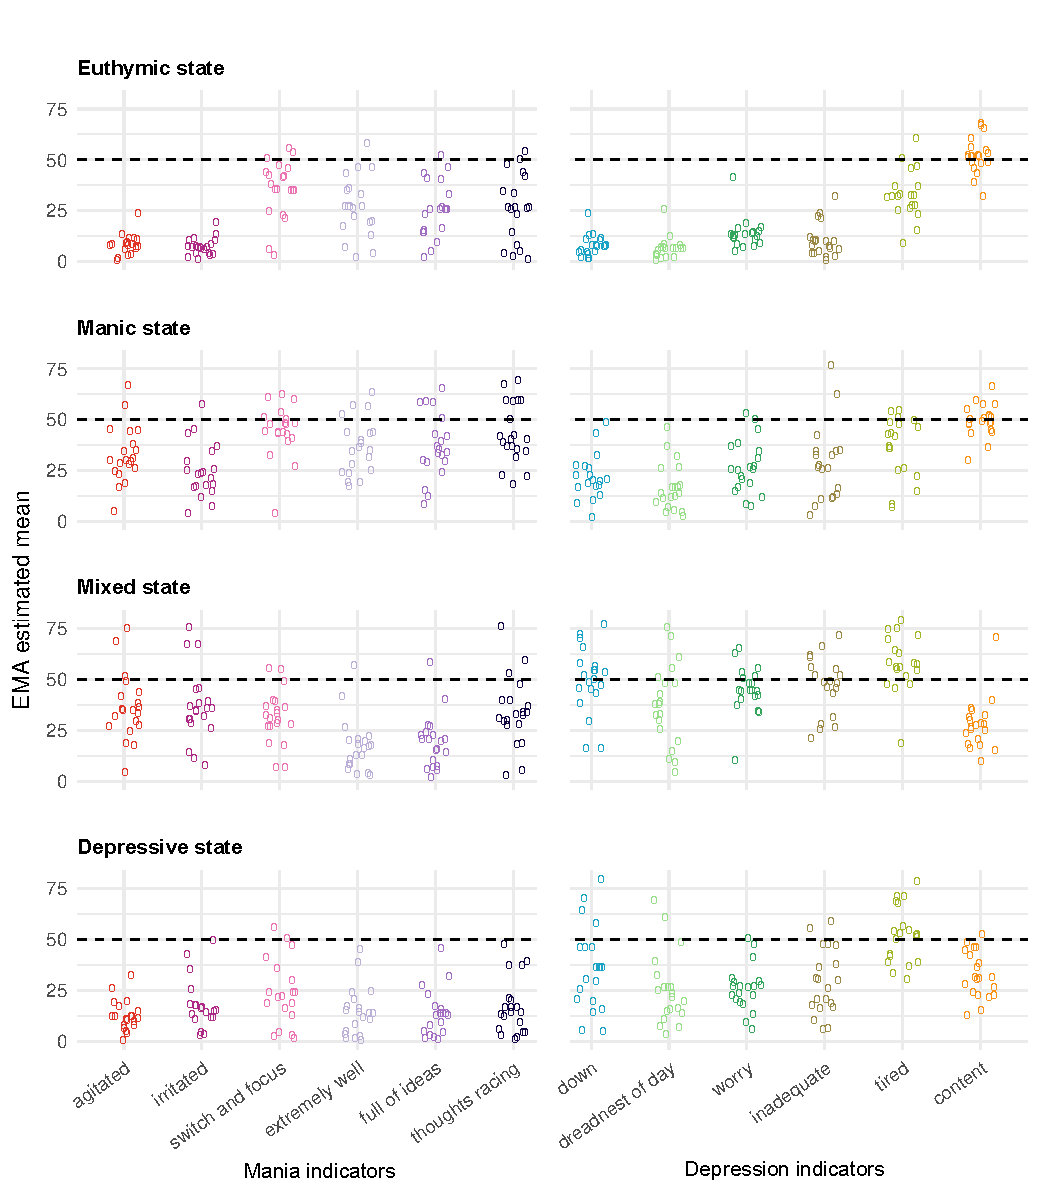
\includegraphics[width=0.8\textwidth]{graphics/ss_emiss.pdf}
  \flushleft
 \footnotesize
 \justifying
 The distribution of all patient-specific estimated emission distribution means for each EMA item is depicted in this figure. On the y-axis, we listed all the EMA items, with the first six being Mania indicators and the next six being Depression indicators. The value of the emission distribution mean is represented on the x-axis. To facilitate comparison, we marked the 50 score value with a dashed line because it is the centre of the possible value scale on all items.
 \label{fig:emiss_ss}
\end{figure}

\subsubsection*{Transitions between hidden Bipolar state: Transition distribution}
The group-level transition probability matrix (TPM) in Figure \ref{combined_ex}A visualizes the dynamics between bipolar states recovered by the \ac{medhmm}. The TPM revealed that the depressive state is the most probable to switch to when being in the euthymic state ($p_{({euth.\rightarrow depr.})}=0.63$ (sd$=0.11$)). When in the manic state, chances of switching to the euthymic ($p_{({man.\rightarrow euth.})}=0.36$ (sd$=0.11$)) and mixed ($p_{({man.\rightarrow mix.})}=0.39$ (sd$=0.15$)) were the largest. From the mixed state, the most probable switch was into the manic state ($p_{({mix.\rightarrow man.})}=0.5$ (sd$=0.15$)). Lastly, the switch to the euthymic state had the largest probability when being in the depressive state $p_{({depr.\rightarrow euth.})}=0.54$ (sd$=0.14$). Since in the \ac{medhmm}, the off-diagonal entries in TPM are redundant, we were also able to compare the outputs across rows (e.g. the group-level chance to switch to the manic state was most likely when the previous state was euthymic). Although the group-level TPM showed average estimated probabilities for the study group, patient-specific deviations to these parameters were present (e.g. the patient-level switching from euthymic to depressive state probability was in $\{0.12-0.94\}$ range). The examples of the patient-specific TPM are also shown in Figure \ref{combined_ex}C. We would like to acknowledge that the group-level TPM estimates of the MHMM were also assessed and revealed slightly different dynamics between mood states transitioning (see Figure \ref{emp_group_trans} in Appendix C for exact transition probability values for the transition matrix of MHMM). 

\begin{figure}[]
\caption{\\The MEDHMM results of group-level and subject-level transition probability matrices and the dwell-time distributions}
 \centering
 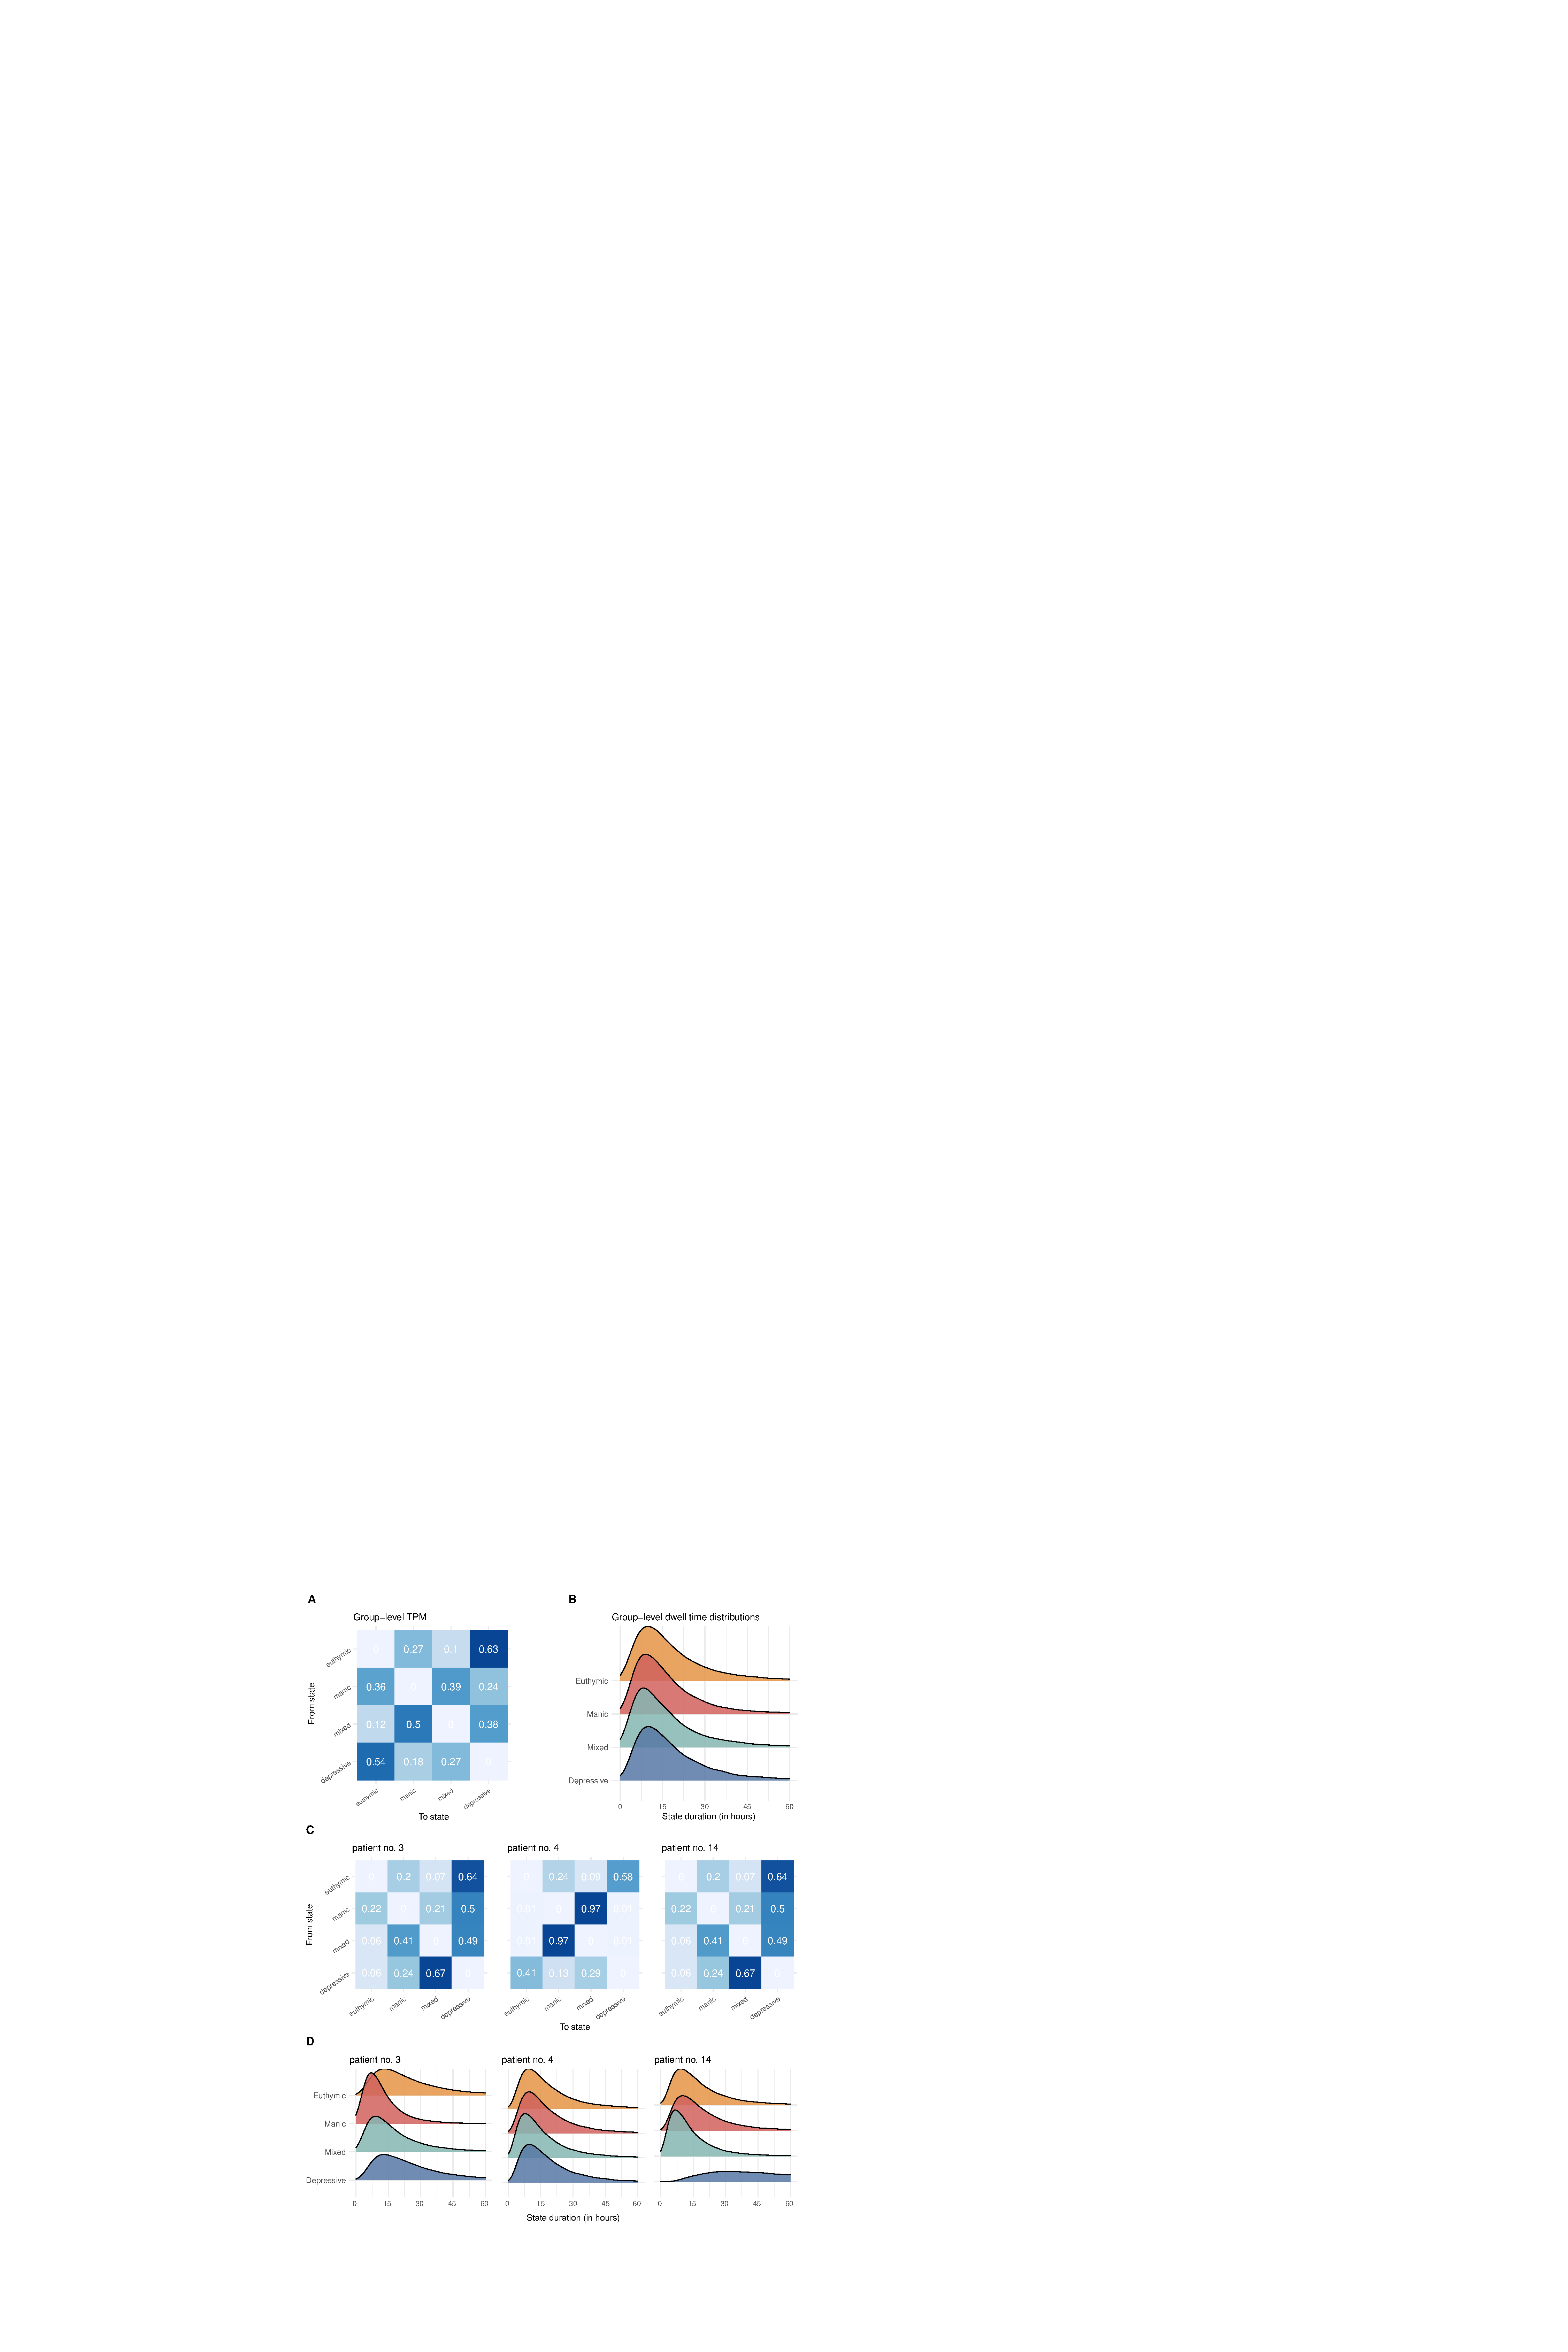
\includegraphics[width=0.75\textwidth]{graphics/empirical_example.pdf}
 \flushleft
 \footnotesize
 \justifying
Panel A shows the group-level transition probability matrix (note that the diagonal entries are equal to $0$); Panel B shows the group-level dwell time distribution for each Bipolar disorder (BD) mood state; Panel C shows the patient-specific (patient-level) transition probability matrices for three patients; Panel D shows the dwell time distributions derived for each BD mood state and are defined for three patients.
 \label{combined_ex}
\end{figure}

\subsubsection*{Bipolar states persistence: Dwell time distribution \& state switching count}
The dwell time distribution revealed that on the group level the expected (median) durations of bipolar states were: $15.10$h(sd$=5.38$h) for the depressive state, $14.61$h(sd$=5.09$h) for the euthymic state, $13.42$h(sd$=4.37$h) for the manic state, and $13.20$h(sd$=5.11$h) for the mixed state (see Figure \ref{fig:gamma_g1} for group-level distributions plotted). The model discovered large patient-specific deviations to the group-level mean, resulting in expected dwell times ranging: from $2.75$h for patient 11 to $13.32$h for patient 7 in the euthymic state; from $2.67$h for patient 17 to $11.25$h in the manic state; from $3.59$h for patient 14 to $6.69$h for patient 1 in the mixed state; and from $2.90$h for patient 7 to $17.90$h for patient 14 (see Table \ref{table_emp_switch} in the appendix for more detailed results). The standard deviations of the patient-specific dwell time distributions were different across subjects and states, with median standard deviations smaller in manic state sd=$\{2.64\text{h}-11.11\text{h}\}$ and more significant in depressive state sd=$\{3.10\text{h}-19.09\text{h}\}$. The count of switches between two different states within a patient observed sequence ranged between $0$ and $115$ switches per subject, and the counts added up to $0$ to $0.273$ proportion of total observations. We refer to Table \ref{table_emp_switch} for more details listed. 

\subsubsection*{Overall performance of MEDHMM when compared to MHMM}
In this part, we would like to draw the reader's attention to two most prominent differences between the MHMM and MEDHMM. 

Firstly, the inspection of overlap of weekly data and decoding derived for each subject for both models (see Figure 11 for example of 3 patients and Figure \ref{decoding_all} in Appendix C for the rest of patient-specific decodings). The MEDHMM resulted in fewer switches in comparison to the MHMM and established more comprehensive states. This result aligned with the outcomes of our simulation study, as the MEDHMM tends to smoothen state decoding more than MHMM. The MHMM decoding was sometimes more unclear with the rapid switches between states. There has been some mismatch in terms of recovered states, for example for patient 4 when the QIDS indicator started to rise from about the 250th observation the MEDHMM marked it as transition from Manic to Mixed state while the MHMM decoded it as transition from Manic to Depressive state through an unclear mixed/depressive mood segment (see middle panel of Figure 11A). Nevertheless, assessing the quality of the models' decoding would require the true sequence of true states for each patient, which is not possible. As an alternative, experts' knowledge in the form of interviews with patients and psychiatrists could be combined with the weekly symptom scores to shed light on this problem. 

Secondly, since the bipolar disorder states durations were assumed log-normal, by using the \ac{medhmm} we could visualise them and estimate for each patient separately. On the contrary, obtaining the direct dwell time distributions for \ac{mhmm} was not possible, and we could only use the self-transition probabilities to model dwell times with approximate exponential distribution. In Figure \ref{exp_ss_dwell} dwell time distributions derived from MHMM and MEDHMM were compared for three patients. We could see that the dwell time distribution of MHMM tended to overlap more than the distributions derived from MEDHMM. This might indicate that possibly some states last longer and the MEDHMM can distinguish them better. The results demonstrated that both models estimated the emission distribution means similarly (see \ref{group_emission_emp} in Appendix C). Given the outcomes from performed simulation study we found that whenever the emission distributions can be recognized, the dwell time distribution in MEDHMM introduced more information to the model resulting in more robust results. In addition, we know that the MEDHMM can distinguish between states when varying dwell times are present in data, which we experience in this dataset. For example, in Figure 12 we could see that for patient 14 the duration of the depressive state had the largest expected duration, which was also in line with the local decoding. That said, 
we believe that the MEDHMM performed better in modelling the dwell times. 

\subsubsection*{Conclusions}
We showed how the Multilevel Explicit Duration Hidden Markov Model can be applied to real empirical data. We modelled the bipolar disorder with four states by applying the MEDHMM that explicitly captured the distributions of mood states' durations. We confirmed the findings from our simulation study by showing that MEDHMM smoothens state decoding and can discover longer dwell times with log-normal distribution. All in all, in our opinion, the MEDHMM worked better in the dwell time estimations as it could capture longer dwell times with more accuracy. We believe that the gains in the accuracy of state decoding could be a promising outcome for practicians. By easing the diagnosis of early warning signals and minimizing the diagnosis to intervention time, this approach could help improve patient outcomes in future. 

\begin{figure}
\caption{\\Temporal alignment between mood states and weekly symptom scores}
    \centering
    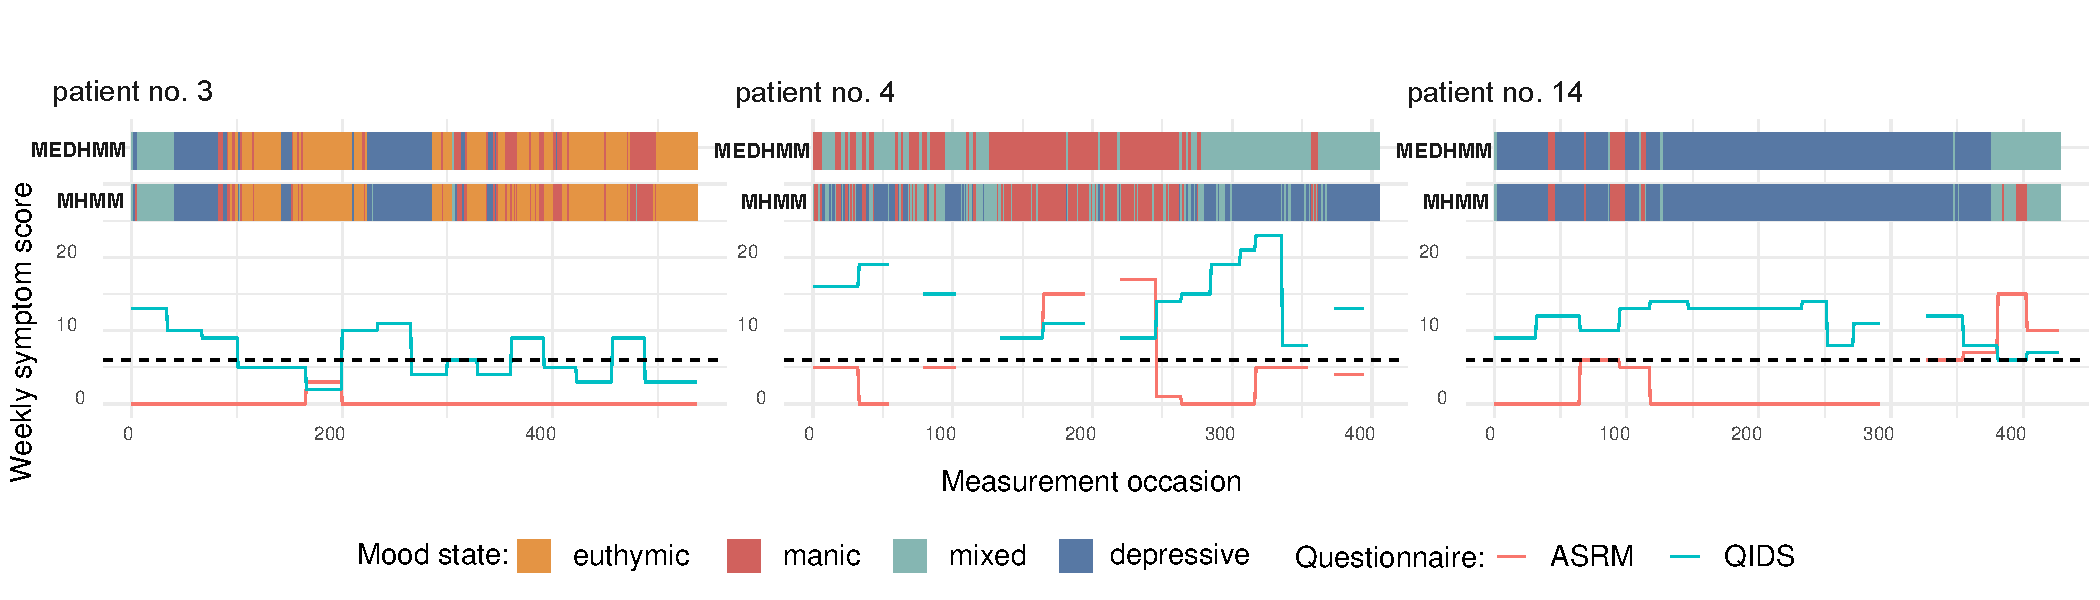
\includegraphics[width=1\linewidth]{graphics/decoding_14.pdf}
    \flushleft
    \footnotesize
    \justifying
    The figure shows local state decoding for the MEDHMM (upper decoding strip) and the MHMM (lower decoding script). The plots are presented for three BD patients to showcase the differences between state decoding. Below strip plots the alignment with the weekly symptom scores on the depressive behaviour indicator (QIDS) and manic behaviour indicator (ASRM).
    \label{quest_vs_decoding}
\end{figure}

\begin{figure}
\caption{\\Derived dwell time distributions for the MHMM and MEDHMM}
    \centering
    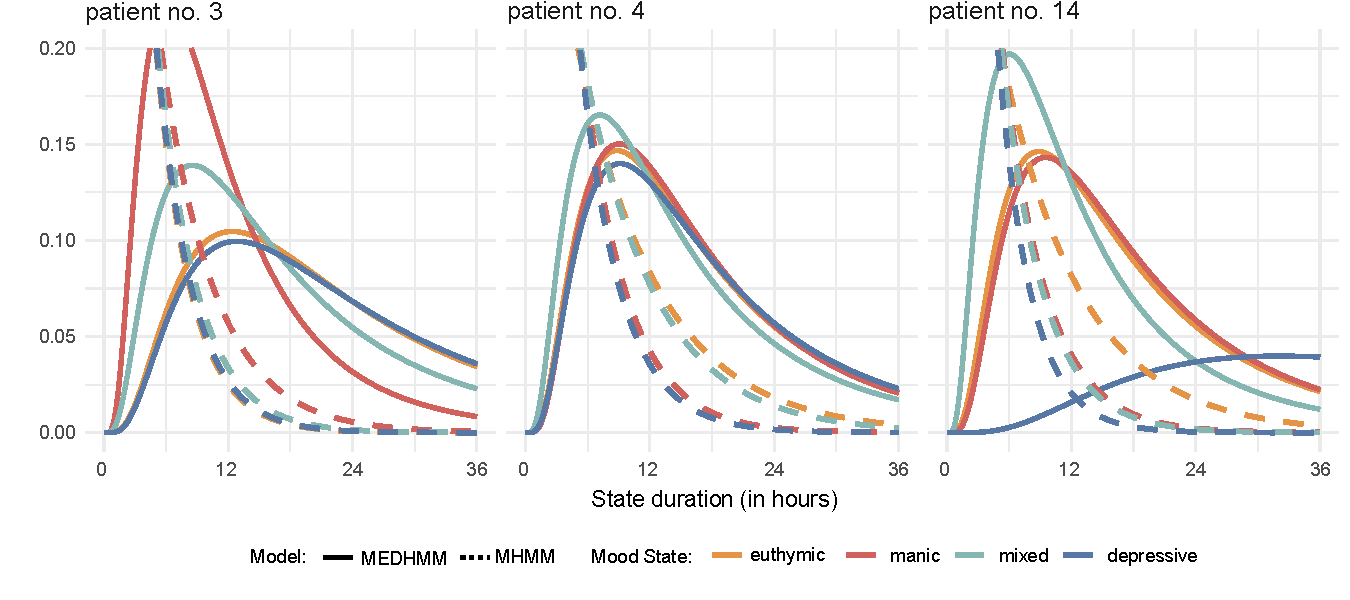
\includegraphics[width=1\linewidth]{graphics/expected_dwell_distr.pdf}
    \flushleft
    \footnotesize
    \justifying
    The plots show the comparison between dwell time distributions derived from MHMM and MEDHMM estimates for three patients from the BD study. The dashed lines represent state-specific exponential distributions that serve as an approximation of the geometric distribution that is assumed to model the dwell time in MHMM. The solid lines represent the dwell time distributions estimated by the MEDHMM that follow the log-normal distribution.
    \label{exp_ss_dwell}
\end{figure}

